\documentclass[12pt]{article}
\usepackage{amsmath}
\usepackage[utf8]{inputenc}
\usepackage{wrapfig}
\usepackage{float}
\usepackage{graphicx} % Required for inserting images
\usepackage{booktabs} % This and below for tables
\usepackage[breaklinks]{hyperref}
\hypersetup{colorlinks=true, linkcolor=Black, citecolor=Black, filecolor=Blue,
    urlcolor=Blue, unicode=true}


\renewcommand{\thesubsubsection}{(\alph{subsubsection})}

\begin{document}


\title{STA4026S Analytics - Neural Networks}

\author{Assignment 1\\
        Laurence Walton\\
        \href{mailto:wltlau003@myuct.ac.za}{wltlau003@myuct.ac.za}
}
\date{August, 2023}

\maketitle

\subsubsection{}
In the context of neural networks the soft-max activation function is used to turn an output layer into a probability distribution where each node has a value between 0 and 1 and the sum of the nodes is 1. This is relevant for multi-class classification problems because with soft-max applied each output node value can be treated as a probability where predictions may correspond to the node with the highest probability, and the error between the predicted probabilities and the true class labels can be used to adjust the network during the training process. The soft-max ensures that the predictions are scaled such that the error accurately reflects the disparities between the predicted probabilities.
The soft-max function in matrix form is:

\[
\sigma(z^n_j) = \frac{exp(z^n_j)}{\sum_{k=1}^q exp(z^n_k)}
\]

Where:
\begin{align*}
z^n_j & : \parbox[t]{0.7\textwidth}{The $j$-th node in the $n$-th training example, i.e. a value from the $q \times N$ output matrix where each row represents a node in the output layer and each column represents a training example} \\
\end{align*}

\subsubsection{}
A potential numerical pitfall in evaluating the cross-entropy error function arises if the predicted probability for a class is 0, as the evaluation would include the logarithm of 0 which is obviously undefined. This is mitigated by using activation functions such as the soft-max, where no predictions can be zero due to exponentiation. However, due to floating point imprecision in software, predictions could be rounded to zero in the soft-max, and therefore cause undefined behaviour in the cross-entropy error function.

\subsubsection{}

Plotting the cross-entropy error obtained on the validation data for varying values of $\nu$ yields:

\begin{figure*}[!ht]
\center
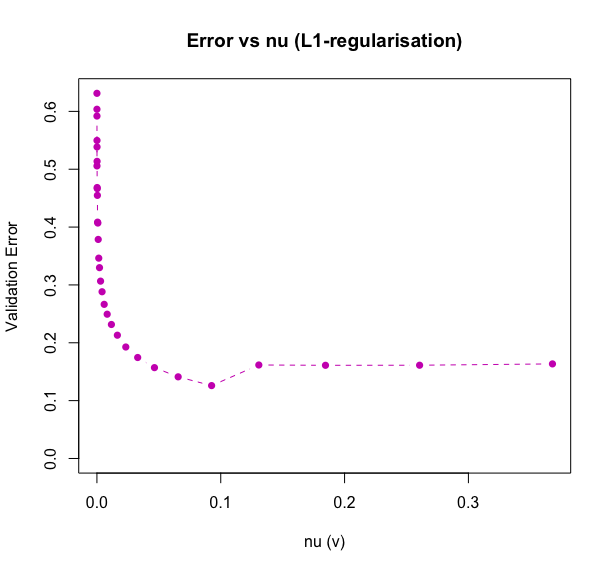
\includegraphics[width=\textwidth,height=0.5\textheight]{question_c_plot.png}
\end{figure*}

Where we find the $\nu$ value of 0.2270106 corresponds to the minimum error (0.1104243).

\subsubsection{}
If we add the results from the neural network with the reLU activation function we obtain:

\begin{figure*}[!ht]
\center
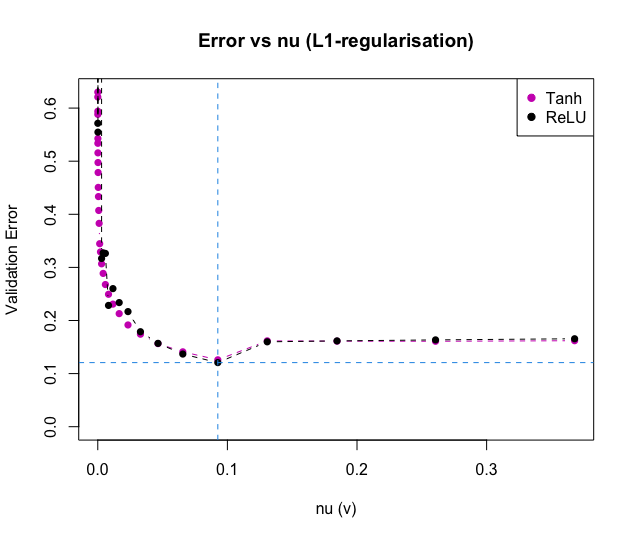
\includegraphics[width=\textwidth,height=0.5\textheight]{question_d_plot.png}
\end{figure*}

\subsubsection{}
\subsubsection{}

\end{document}
